\section{Presentation Logic Layer}

%What pages will be present in your project? briefly indicate how your web site will be organized

Lyrify+ has two main areas: the user area and the artist area. Both are accessible through the login page where the user can decide to login as an user or as an artist, according to their role. The accessible pages for users can only be seen by users, idem for the artist, the only common page for both type of users is the login page.
Now we define the pages to be developed in Lyrify+.
\begin{itemize}
    \item Login / Register page: first shown page to all users. They will be able to choose to login as an user/artist or to register as a new user/artist.
    \item Homepage: main page showed when a user's is logged in.
    \item User profile page: page that shows the user personal data and account options.
    \item Artist profile page: page that shows the artist's personal data, upload options and account options.
    \item Artist page: page that shows the public data of an artist, including biography, songs and albums.
    \item Upload song page: page where it's possible to upload songs, only accessible by verified artists.
    \item Upload album page: page were it's possible to upload albums, only accessible by verified artists.
    \item Library page: page showing users' playlists, liked songs and added albums.
    \item Song page: page that shows information about the song.
    \item Playlist/Album page: page that shows information about the playlist or the album.
\end{itemize}


%For the main pages put a mockup and describe it in detail.

\subsection{Login / Register Page (Interface Mockup)}

\begin{figure}[h!]
\centering
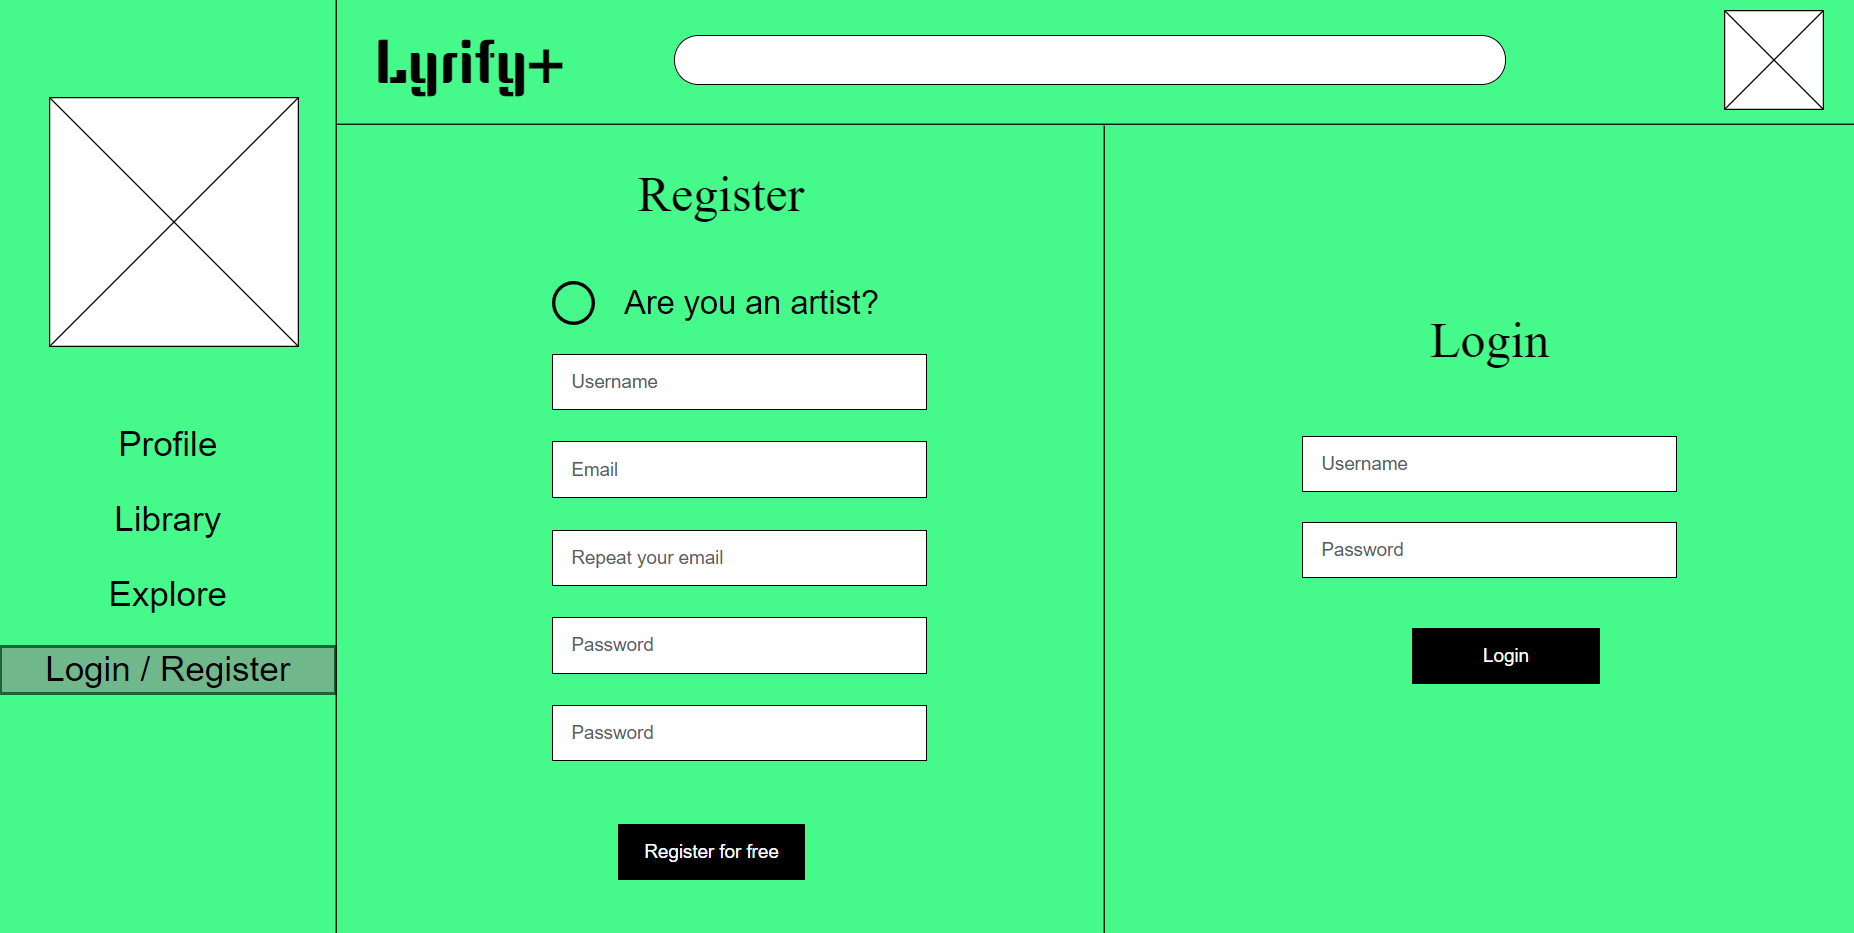
\includegraphics[width=0.9\textwidth]{sections/PLL/LoginPageMockup.png}
\caption{Login page}
\end{figure}

The Login/Register page is the first page that appears when accessing Lyrify+ on the browser. Here, the user can either register as a new user or artist or login if they already have an account. 
For the register form, the user will be asked to: mark the radial button in case he wants to create an account as an artist, enter an username, an email and confirm it and a password also with its confirmation. The username to be provided can have as much as 50 characters, the email is required to have the typical email schema and the password will be required to be between 8 to 25 characters. By clicking the 'Register for free' button the user's credentials will be added to our database and the user will be redirected to the homepage, or to the artist profile page in case they registered as an artist.  
For the login form the user is required to enter their credentials (username and password) and then click the 'Login' button that will check if the credentials are correct and if they are in our database. Once completed the users will be redirected to the homepage and the artists will be redirected to the artist profile page.

\subsection{Homepage (Interface Mockup)}

\begin{figure}[h!]
\centering
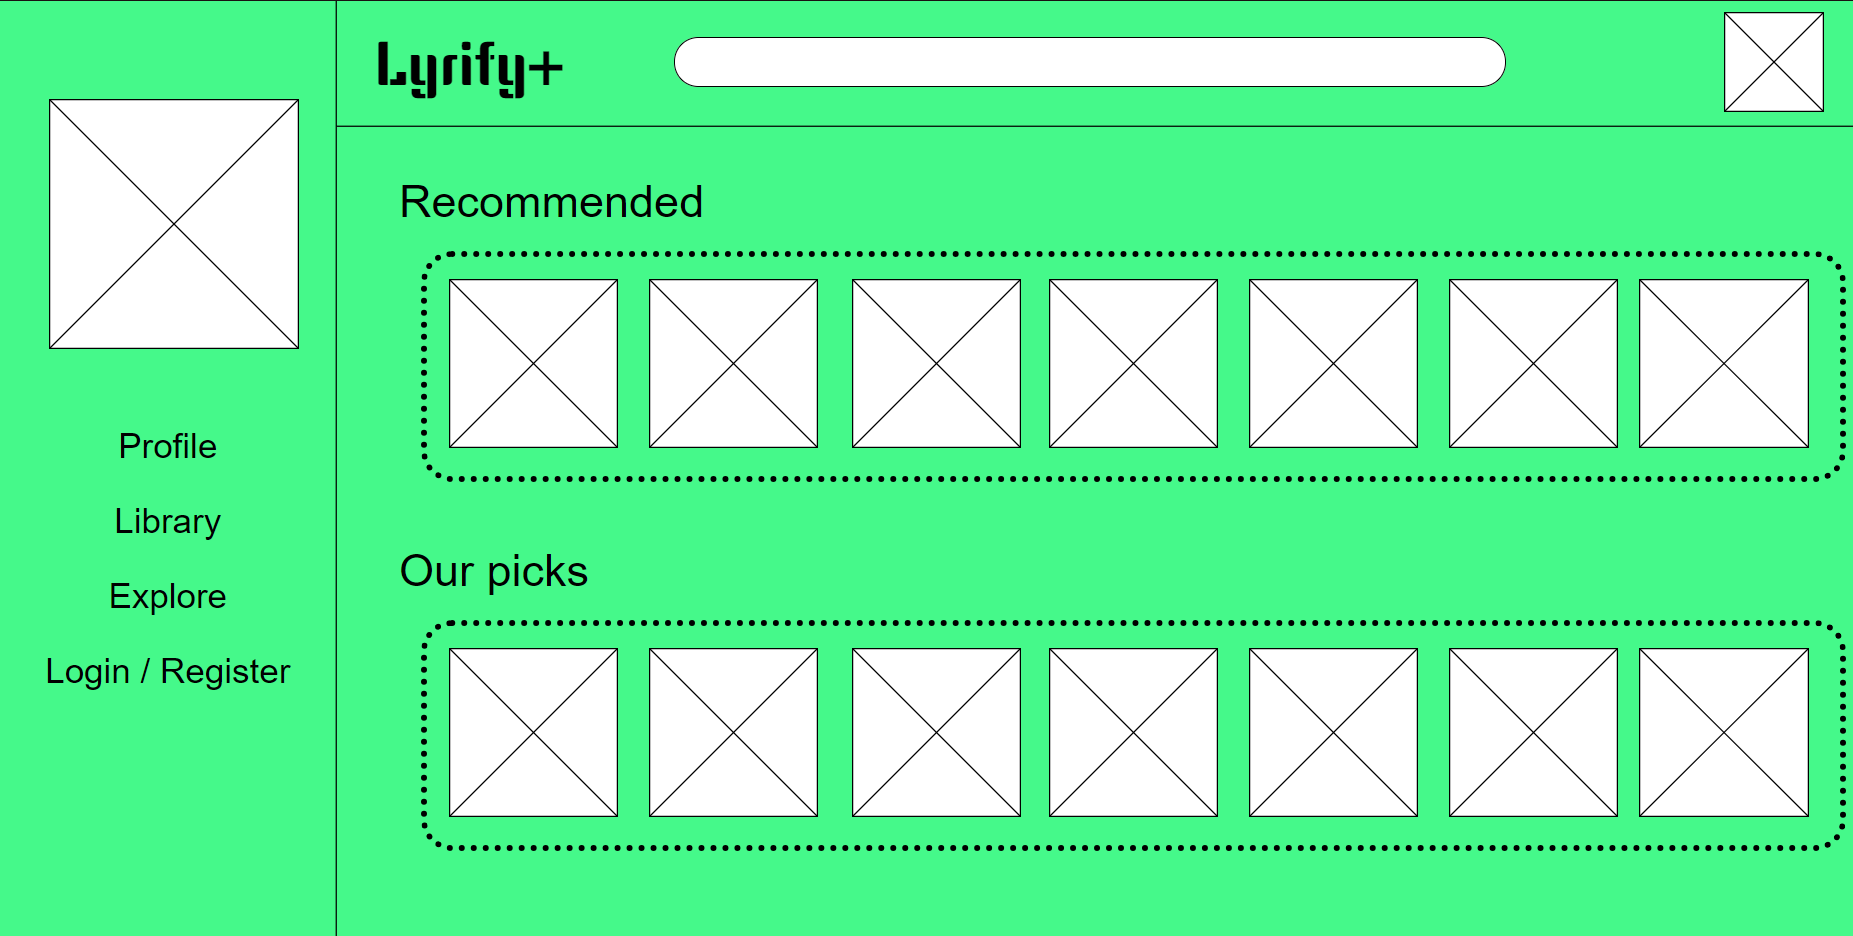
\includegraphics[width=0.9\textwidth]{sections/PLL/HomePageMockup.png}
\caption{Homepage}
\end{figure}

On the Homepage, the screen will show a menu on the left side that includes the app's logo, a button for accessing the user's profile, the library page, an explore page for discovering new songs and a logout button in case they want to leave the application. On the top row they will be able to see the app's name, a search bar for searching songs in the database and their profile photo on the top right corner to show that they are logged in.
Then, in the center of the page, the user will see two main rows showing our recommendations, picked by the algorithm: as of now the algorithm reads from the database songs and albums not older than 1 year, but this could be changed in the future.

\subsection{User Profile Page (Interface Mockup)}

\begin{figure}[h!]
\centering
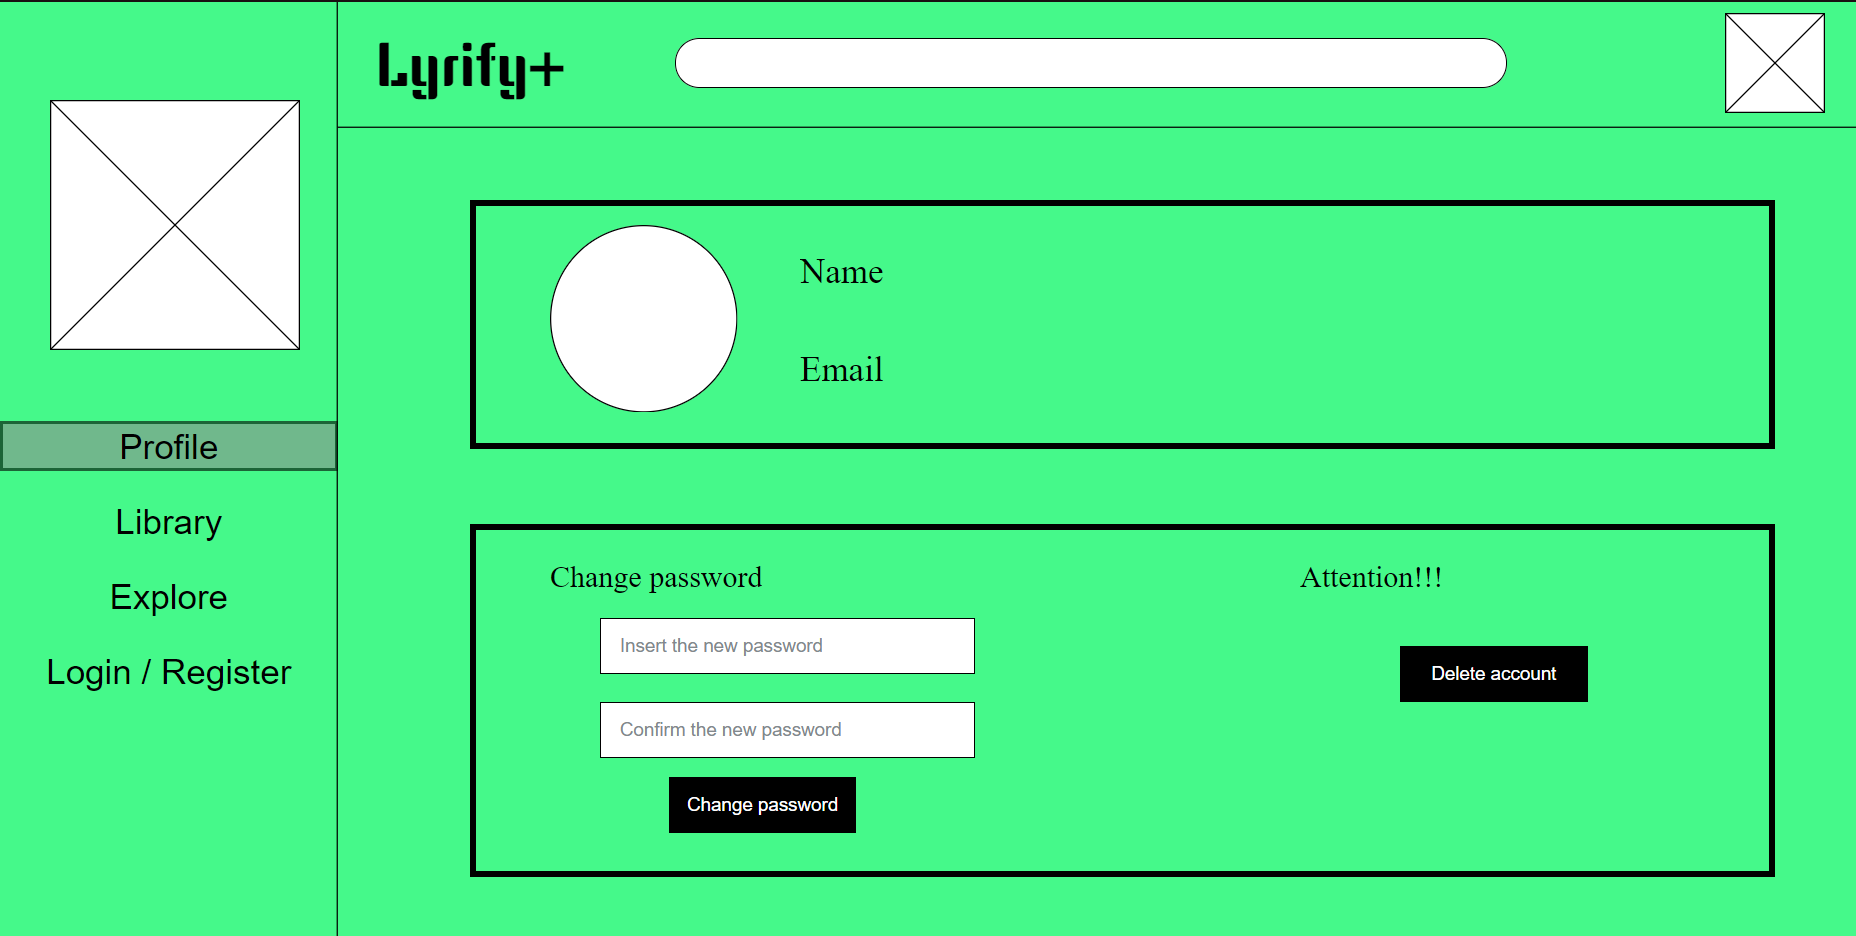
\includegraphics[width=0.9\textwidth]{sections/PLL/ProfilePageMockup.png}
\caption{User profile page}
\end{figure}

On the user's profile page, the menu on the left side will be repeated but with the 'Profile' button darkened to indicate that the user is in that page. Then, the top row is also shown including the app's name, search bar and profile photo. The center of the page will be divided in two parts, the user's information part and the account settings part.
For the user's information part, the profile photo will be displayed in a bigger size along with the username and the mail.
For the account settings part, there will be an option for changing the password by filling both fields and then clicking on the 'Change password' button, that will update our database with the new credentials for the user. In addition, in case the user no longer wants to keep using our app, there will be a 'Delete account' button that will delete all the user's data from our database and will redirect the user to the Login / Register page. 

\subsection{Artist Profile Page (Interface Mockup)}

\begin{figure}[h!]
\centering
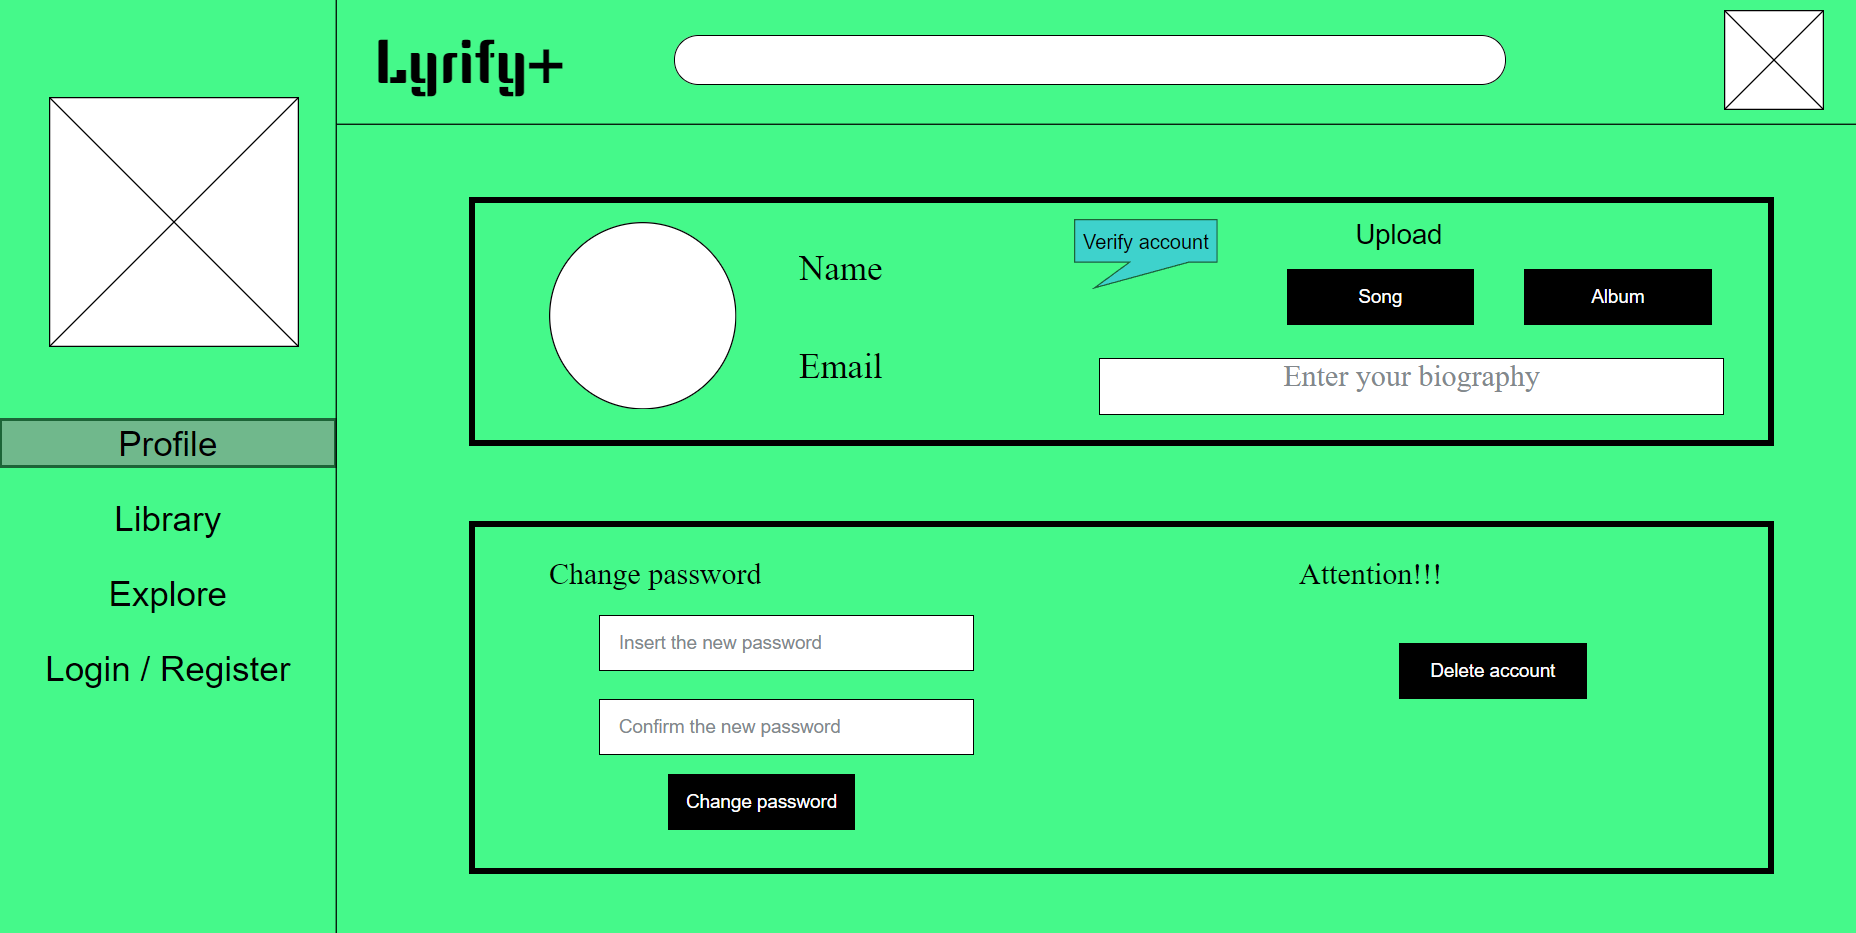
\includegraphics[width=0.9\textwidth]{sections/PLL/ProfilePageArtistMockup.png}
\caption{Artist profile page}
\end{figure}

On the artist’s profile page, the menu on the left side and the top row will remain the same as in the user’s profile page. The center of the page will be divided in two parts, the artist’s information and options part and the account settings part. 

For the artist’s information part, the profile photo will be displayed in a bigger size along with the username and the mail. In addition, it includes the verify button, that will disappear once the account is verified; and the buttons for uploading either songs or albums and the biography area for the artist to describe himself.

For the account settings part, we maintained the same fields as in the user’s profile page, an option for updating the password and for deleting the account.

\subsection{Artist Page (Interface Mockup)}

\begin{figure}[h!]
\centering
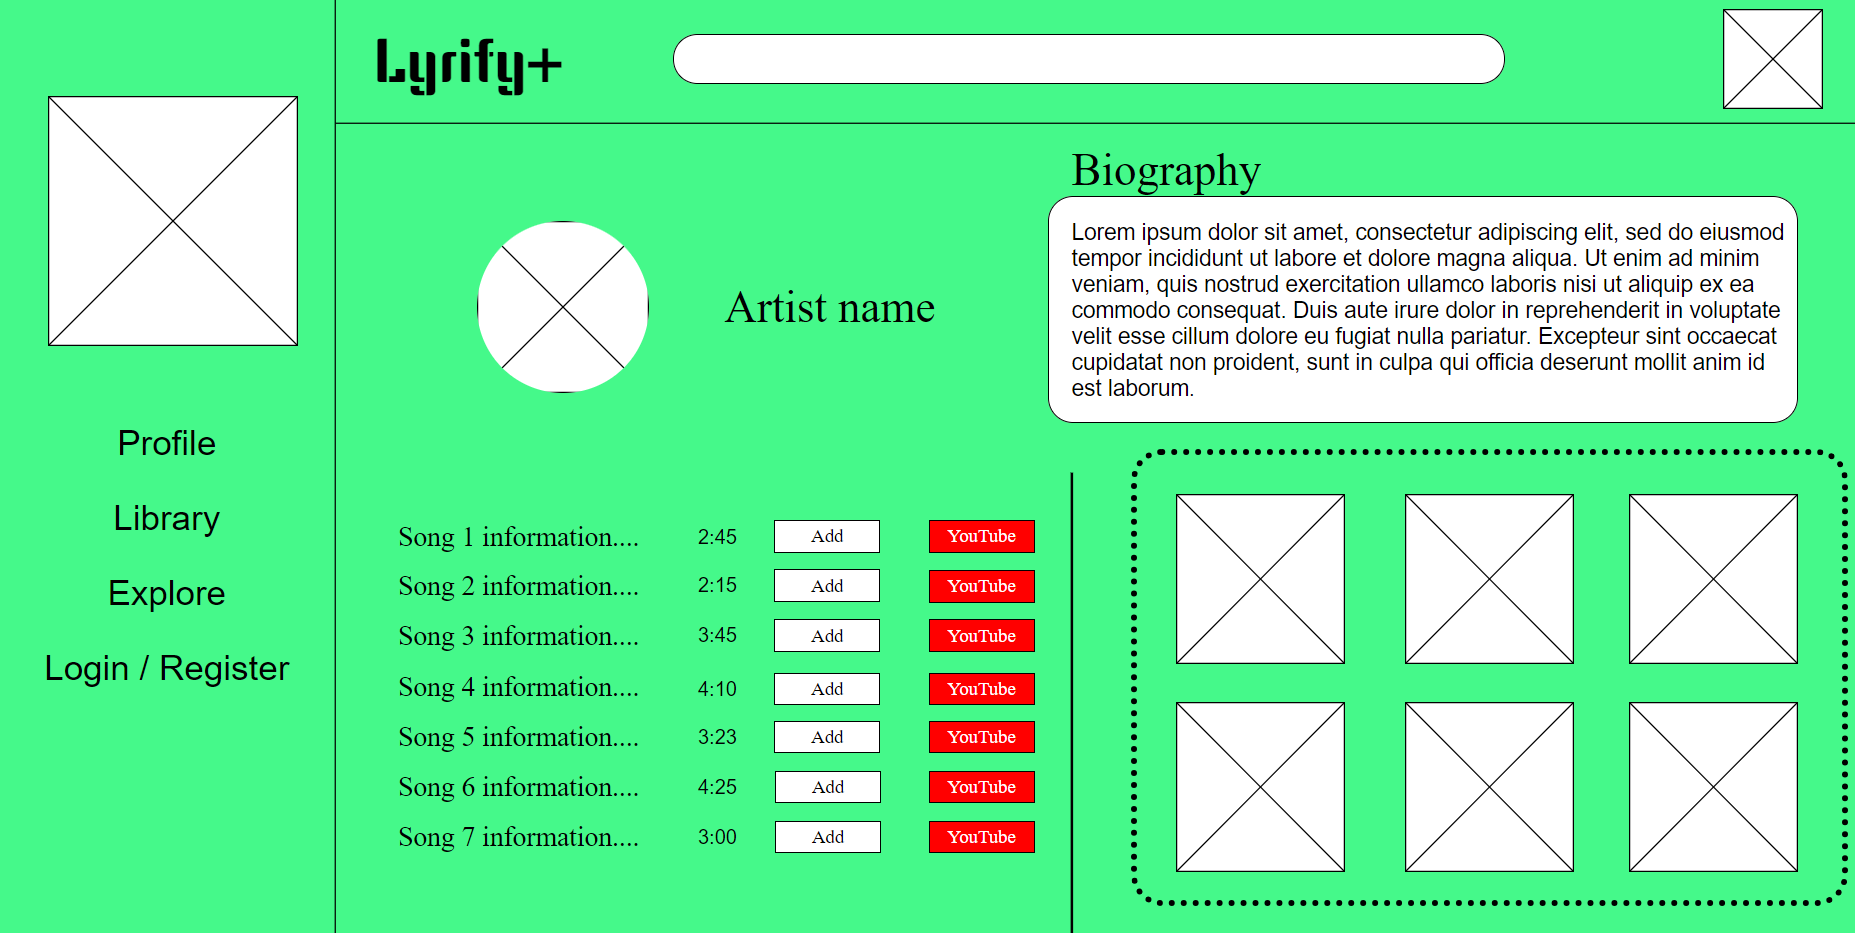
\includegraphics[width=0.9\textwidth]{sections/PLL/ArtistPageMockup.png}
\caption{Artist page}
\end{figure}

For the artist’s page, which is not the same as the artist’s profile page, it will be shown the public information from the artist. We maintain the design for the side panel and the top row as for the other pages. Then, in the center of the page the following information is shown:  

\begin{enumerate}
    \item Top left corner: Artist’s name and profile photo
    \item Top right corner: The artist’s biography
    \item Down left corner: A list with the artist’s songs showing the name of each of them, their duration, a button for adding them to a playlist and a YouTube button to redirect the user to the song’s YouTube video. In addition, by clicking on the name of the song, the user will be redirected the song’s information page, which will include the lyrics of it. 
    \item Down right corner: A grid with the artist’s released albums showing only the album’s cover, that by clicking on them will redirect the user to the album’s information page, with their respective information and songs belonging to the album.
\end{enumerate}


\newpage
\subsection{Upload Song Page (Interface Mockup)}

\begin{figure}[h!]
\centering
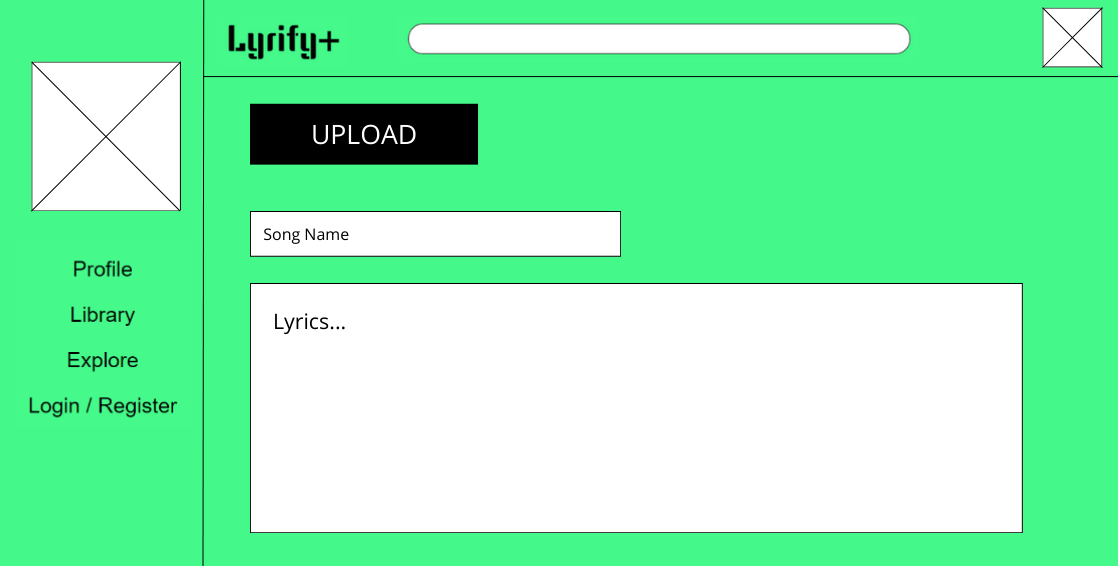
\includegraphics[width=0.9\textwidth]{sections/PLL/UploadSongMockUp.png}
\caption{Upload song page}
\end{figure}

This page is simpler as it has the typical design of the others for the side and the top row. In the center of the page, we can find the upload button, for adding the song to our database, and two fields for entering the song’s name and lyrics. 

\subsection{Upload Album Page (Interface Mockup)}

\begin{figure}[h!]
\centering
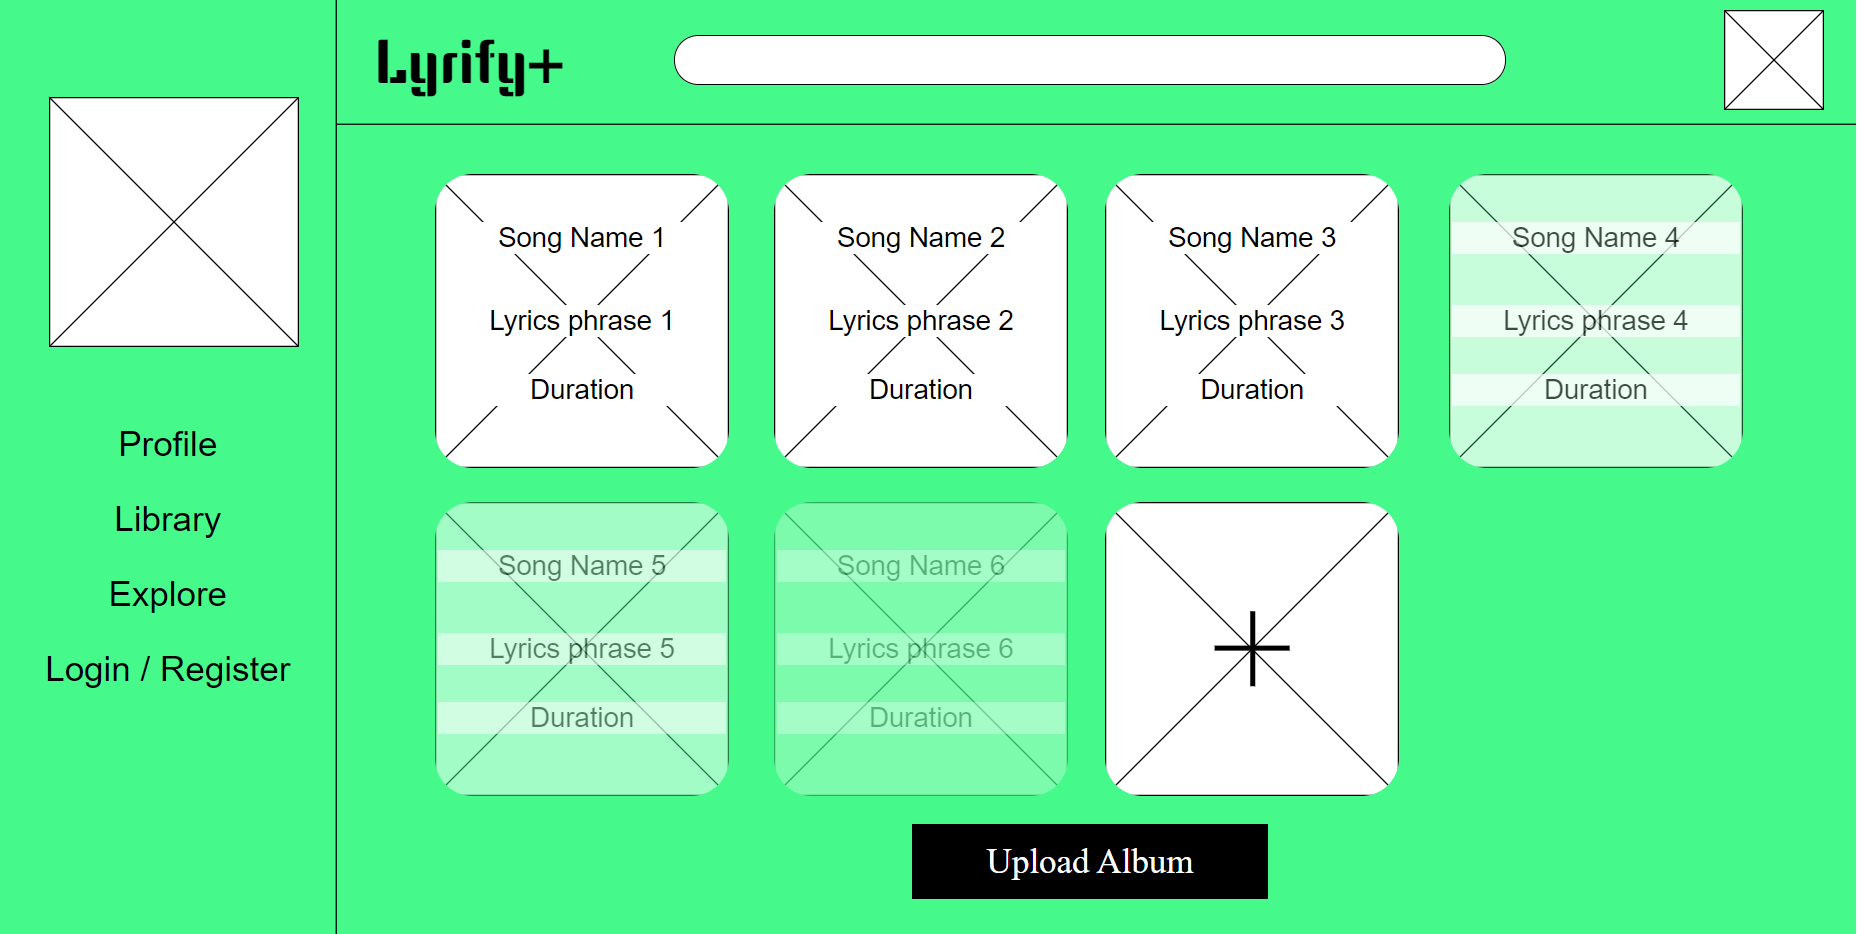
\includegraphics[width=0.9\textwidth]{sections/PLL/UploadAlbumMockUp.png}
\caption{Upload album page}
\end{figure}

This page is simpler too as it has the typical design of the others for the side and the top row. In the center of the page, we can find some squares that represents the songs added to the album. The page will begin only with the square that has a plus in the center. By clicking on it, the page will redirect you to the upload songs page in order to enter the rest of the song’s information. When done, the page will redirect you back to the album, and one square with the basic info of the song the artist just entered will be displayed, and next to it the add song square. This way the page will be filling up with the songs the artist enters. Once the album is completed, the artist will need to click on the ‘Upload album’ button to save it in our database and will be redirected to the artist’s profile page.

\subsection{Library Page (Interface Mockup)}

\begin{figure}[h!]
\centering
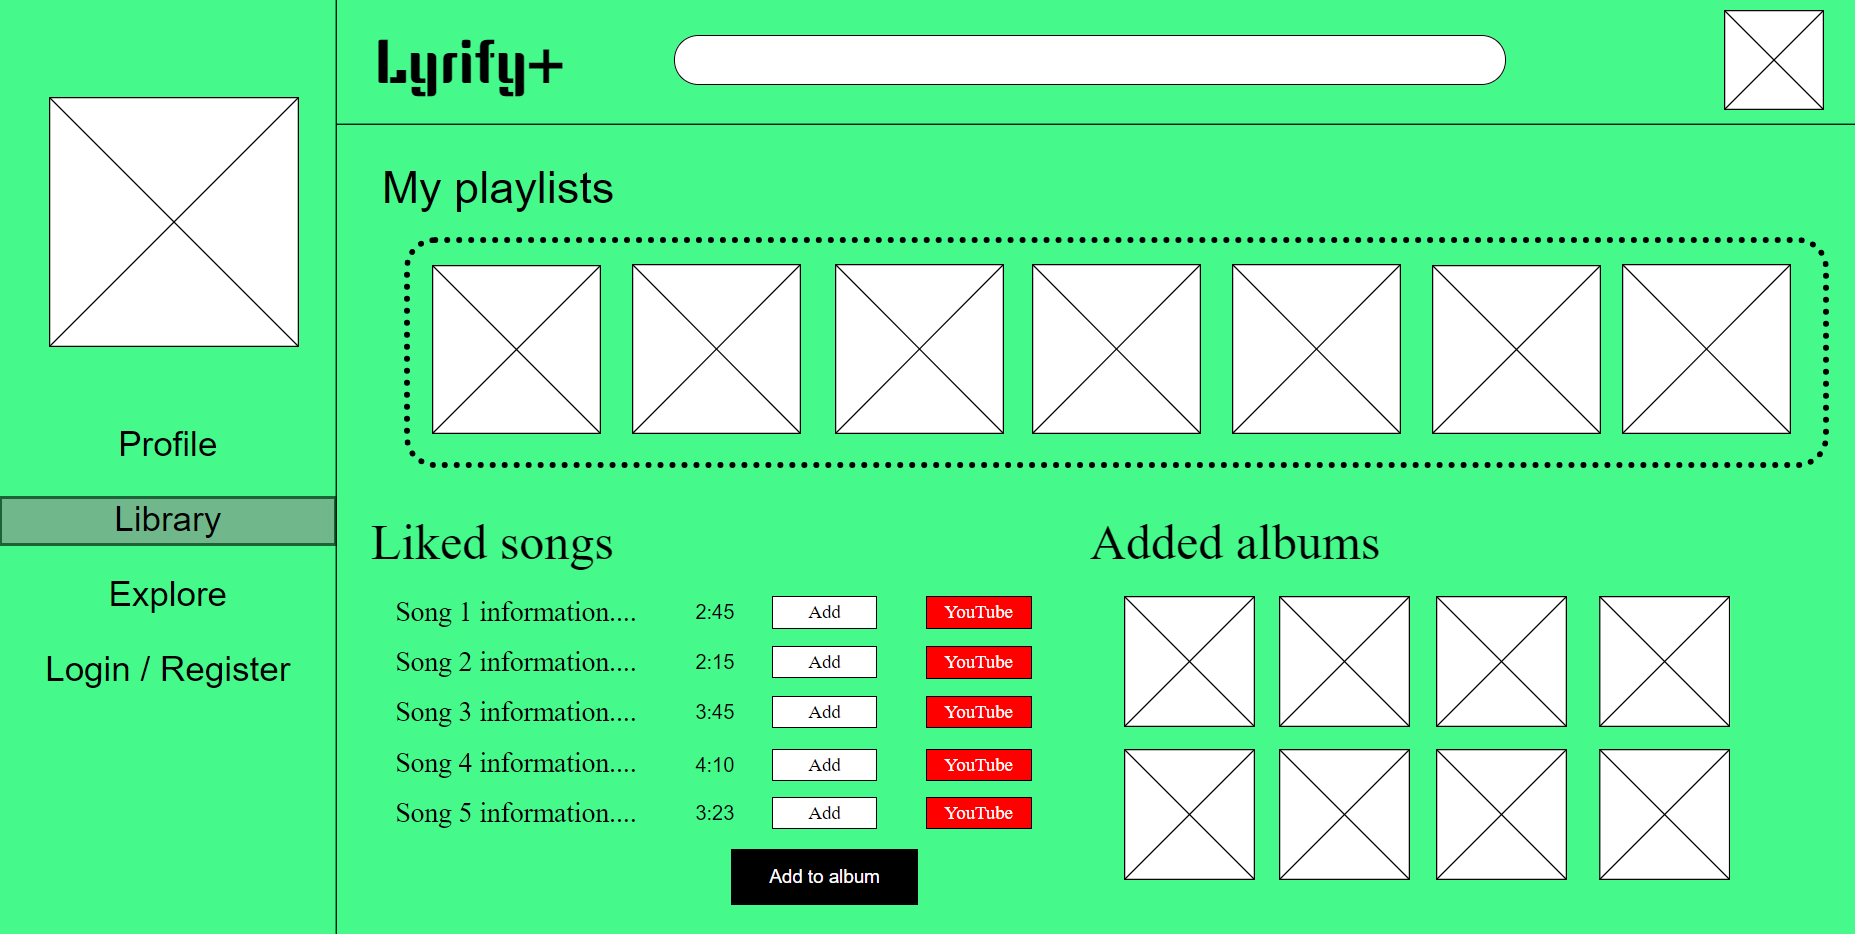
\includegraphics[width=0.9\textwidth]{sections/PLL/LibraryPageMockup.png}
\caption{Library page}
\end{figure}

For this page, we still maintain the design for the side and top panels, with the exception on the darkened ‘Library’ part to show that the user is on the library page. In the center of the page, there will be displayed a row with the user’s playlist that will be empty in the beginning and will grow as the user makes them. On the bottom part, the user will be able to see a small list of the liked songs, showing the names, duration, possibility to add to a playlist and YouTube video button; on the other side a list of the added albums will be displayed too, showing only the albums’ covers. 

\subsection{Song Page (Interface Mockup)}

\begin{figure}[h!]
\centering
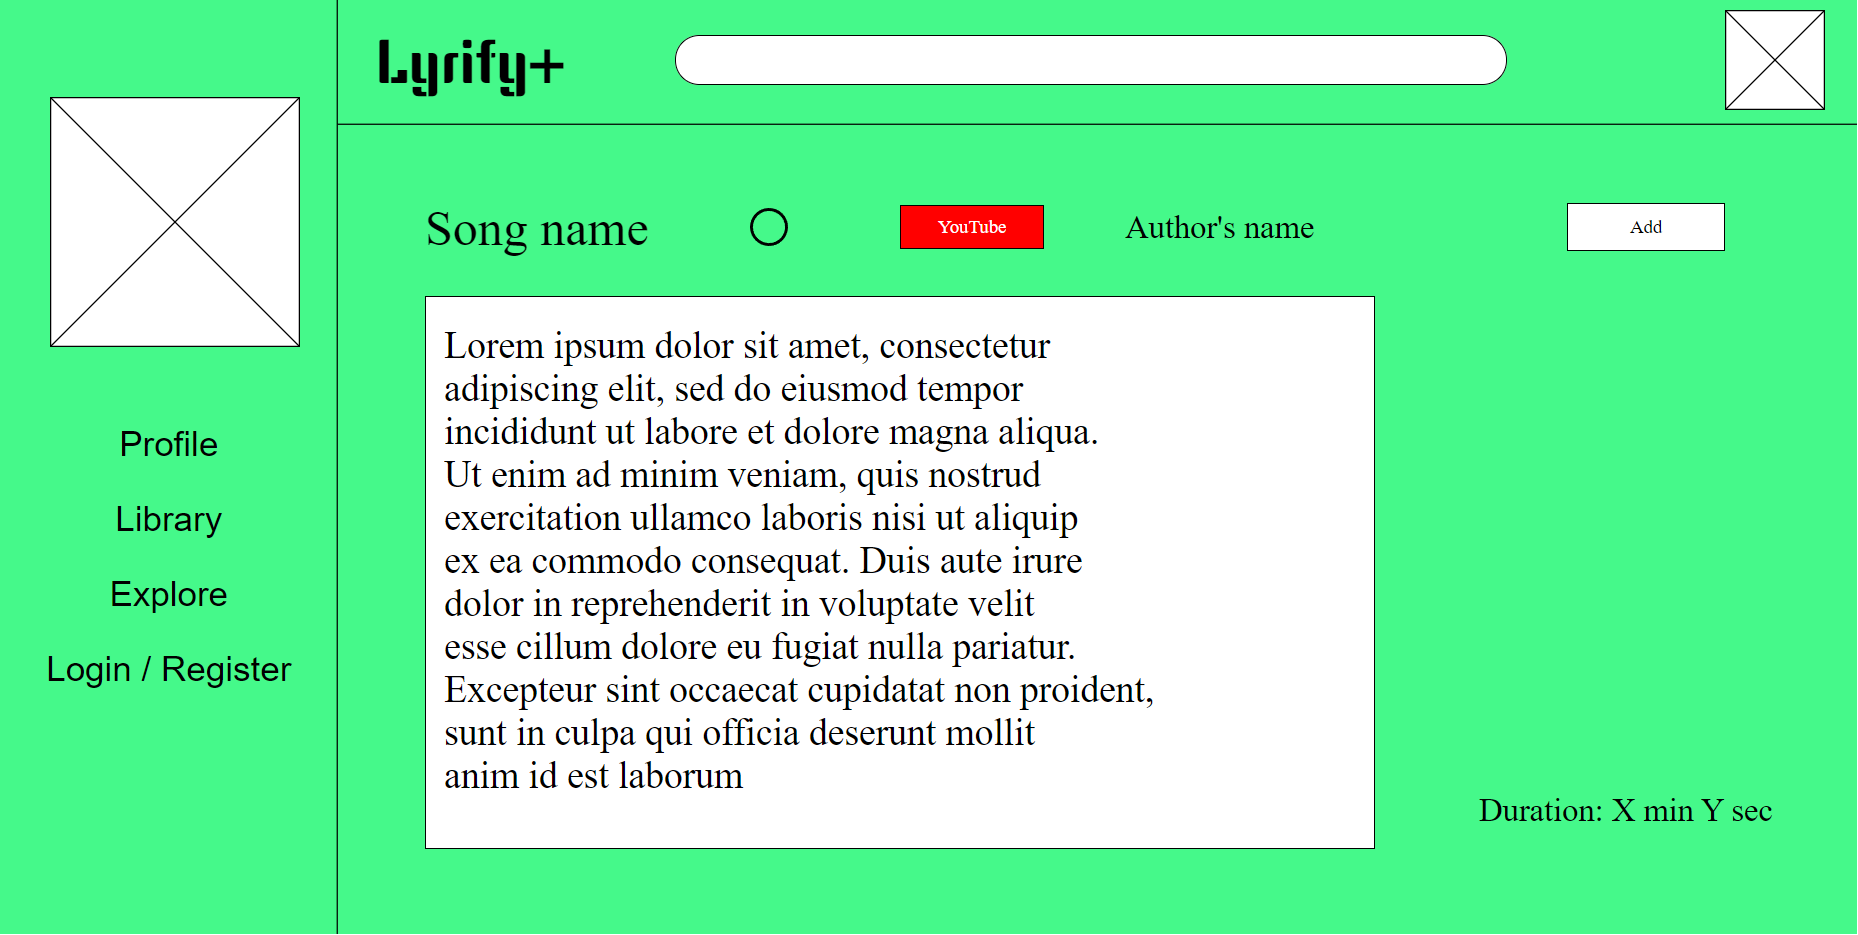
\includegraphics[width=0.9\textwidth]{sections/PLL/SongPageMockup.png}
\caption{Song page}
\end{figure}

For the song page, there will still be the top and side panels as in the other pages. In the center, the user will be able to see the name of the son, next to it a button to like the song, the YouTube video button, author’s name and a button for adding the song to a playlist. Below this, the lyrics of the song will be displayed, and on the bottom right corner the duration of the song will be shown.

\subsection{Playlist / Album Page (Interface Mockup)}

\begin{figure}[h!]
\centering
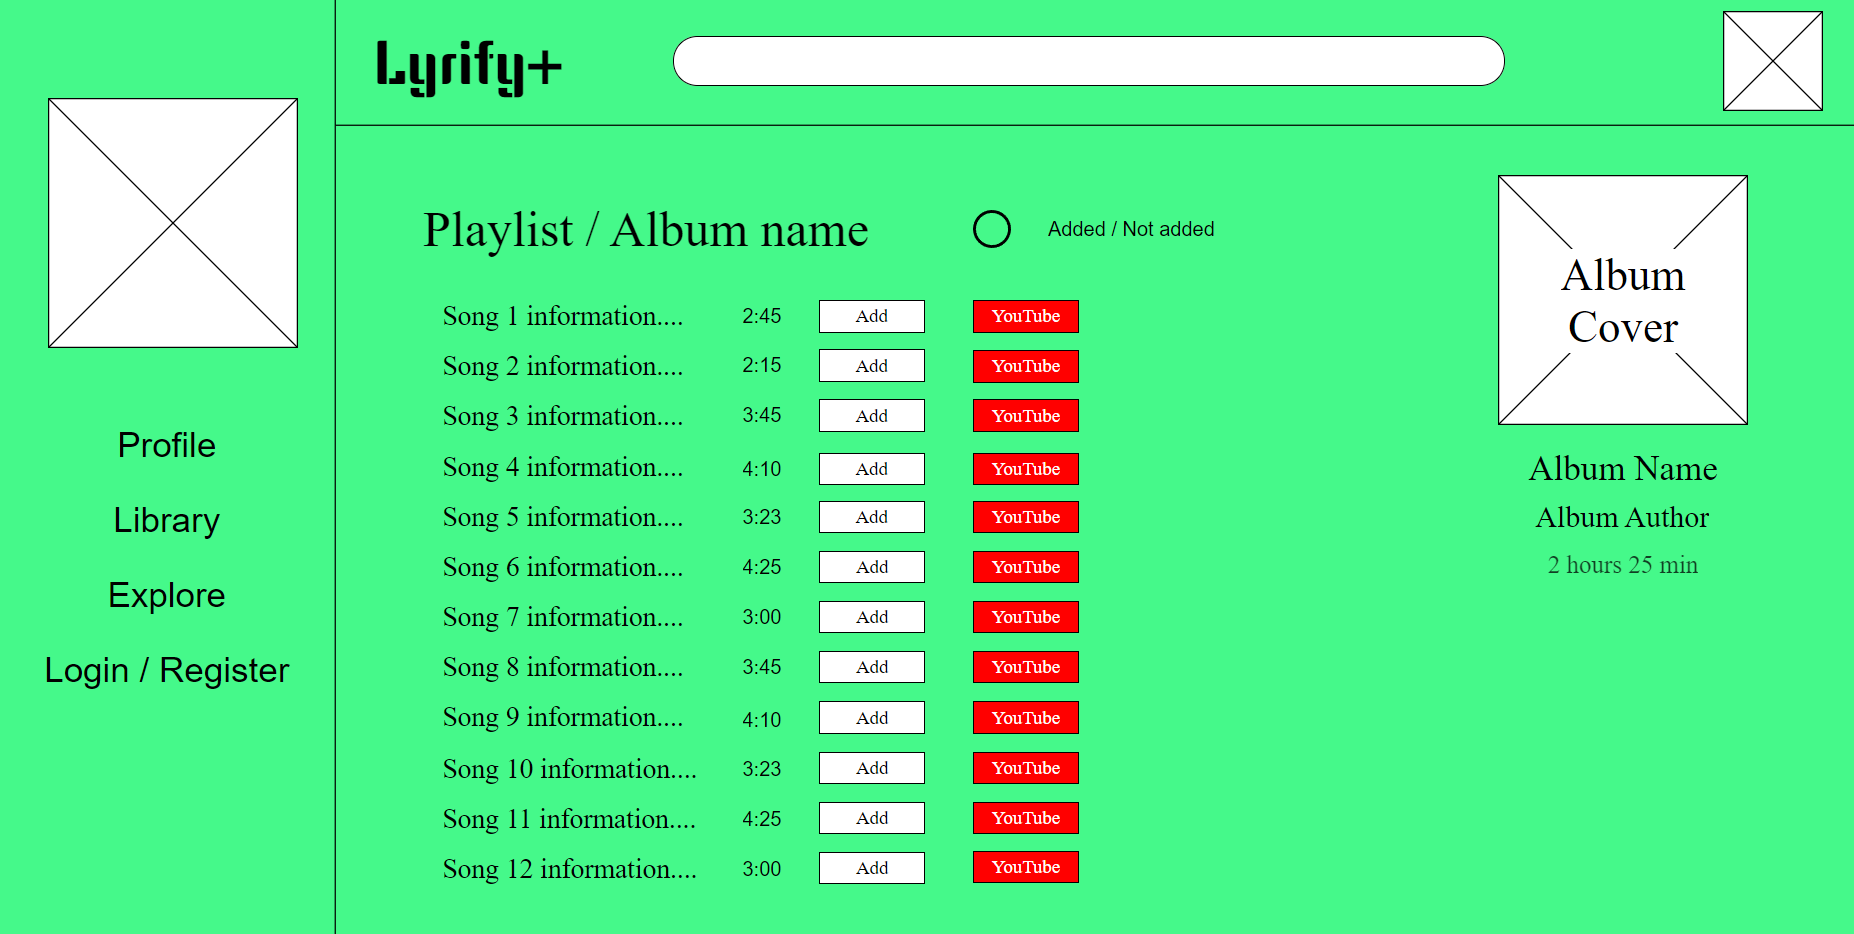
\includegraphics[width=0.9\textwidth]{sections/PLL/PlaylistPageMockup.png}
\caption{Playlist / Album page}
\end{figure}

For this page, the general design is maintained as always, regarding the side and top panels. Then, the info displayed in the page will depend on from where it is opened, because it will display info for playlists and albums.

As an album page, the album’s name will be displayed on top, next to it, an added button will appear selected in the case the album is added by the user or empty in case the user has not selected yet the album. On the right side, the album’s cover photo, name, author and complete duration will be displayed. And, in the center of the page, the list of songs belonging to the album will be displayed, showing the songs’ names, durations, add buttons and YouTube video buttons.

As a playlist page, the page will show the playlist’s name, and the list of songs with all the respective information regarding the songs.
